\ifdefined\XeTeXversion\else\pdfoutput=1\fi
\documentclass[10pt,twocolumn]{article}

\usepackage[margin=0.75in]{geometry}
\usepackage{booktabs}
\usepackage{microtype}
\usepackage{amsmath}
\usepackage{graphicx}
\usepackage[hidelinks]{hyperref}
\usepackage[numbers,sort&compress]{natbib}

\newcommand{\system}{DareFightingICE}
\newcommand{\lewm}{LeWM}
\newcommand{\dreamer}{DreamerV3}
\newcommand{\pets}{PETS}

\title{Which World Model Is the Best Fighter?\\
\lewm{} vs.\ \dreamer{} vs.\ \pets{}}
\author{Chinh Nguyen-Thanh\\
\texttt{nguyenthanhchinh96@gmail.com}}
\date{}

\begin{document}
\maketitle

\begin{abstract}
This short report compares three trained world-model controllers in
\system{}: pixel-based \lewm{}, vector-based \dreamer{}, and vector-based
\pets{}.  Across 135 reported lockstep rounds, \dreamer{} beat \lewm{} 32--13
and \pets{} 45--0; \lewm{} beat \pets{} 28--17.  \dreamer{} also had the
lowest mean decision latency.  Per-match results vary: the three
\dreamer{}--\lewm{} matches ran 11--4, 14--1 and 7--8, so the pooled total
overstates how settled that pair is.  These are preliminary results for fixed
controllers, not evidence that one world-model architecture is generally
better: inputs, training data, planning budgets, and player-side coverage
differ, and none of the three is compared against the platform's standard
search-based agent.
\end{abstract}

\section{Introduction}

This personal side project is motivated by LeWorldModel
\cite{maes2026lewm}.  We adapt its visual world model to a fighting game
and compare the resulting controller with \dreamer{} and \pets{}.
World models learn predictive representations for control
\cite{ha2018worldmodels}.  We compare complete controllers in \system{},
without proposing a new algorithm.

\section{The Game and Competition}

FightingICE is a Java-based fighting-game AI research platform maintained
by Ritsumeikan University's Intelligent Computer Entertainment Lab.
Its competition invites controllers to fight other agents and supports
Python interfaces and visual controllers \cite{fightingicePlatform}.
\system{} extends FightingICE with richer sound support.  The 2022
\system{} competition at the IEEE Conference on Games introduced sound-design
and audio-only AI tracks, motivated by accessibility for visually impaired
players \cite{khan2022darefightingice}.  Our experiment uses the platform,
not those competition rules: it is a local pixel/state-vector comparison,
not an official entry or an audio-only benchmark.

Search-based agents are the established reference point on this platform:
the shipped MctsAi sample agent plans directly in the game's forward
simulator rather than in a learned model \cite{yoshida2016mctsai}, and
variants of it have been competitive entries for years.  We do not
compare against it here.  All three of our controllers are learned world
models evaluated only against each other, so the numbers below locate them
relative to one another and not relative to the platform's standard
baseline.

\paragraph{Why this game?}
It provides direct head-to-head outcomes, observable HP changes, and both
image and structured-state interfaces in the same environment.  This makes
it a practical small-scale test bed for a visual predictive model, a learned
latent policy, and an explicit dynamics planner.  The shared engine keeps
the task consistent, although different input modalities prevent a
controlled comparison of representation quality.

\section{The Three Controllers}

Figure~\ref{fig:controllers} summarizes the observation-to-action path
for each controller.  All model weights remain fixed during evaluation.

\begin{figure*}[t]
\centering
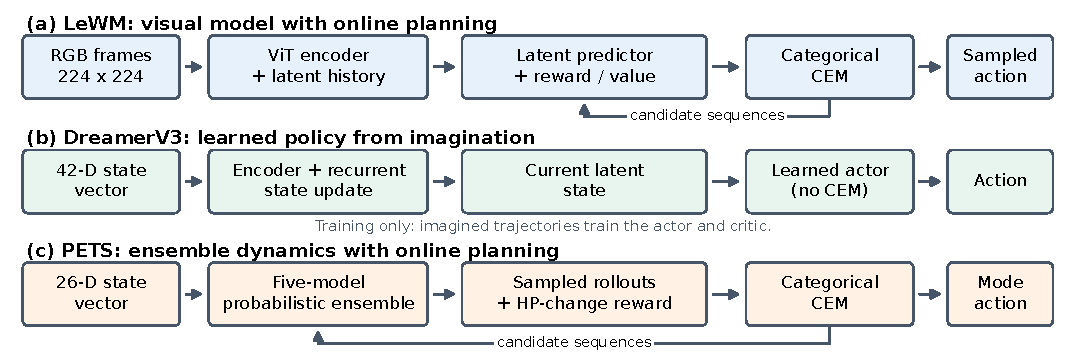
\includegraphics[width=\textwidth]{figures/controller_diagrams.pdf}
\caption{The three evaluated controllers.  Solid forward arrows show the
observation-to-action path; the lower arrows show candidate sequences
proposed by CEM for model-based scoring.  \lewm{} and \pets{} search online,
whereas \dreamer{} uses an actor trained on imagined trajectories.}
\label{fig:controllers}
\end{figure*}

\paragraph{\lewm{}: visual prediction and planning.}
LeWorldModel (\lewm{}) learns an action-conditioned joint-embedding world model rather
than reconstructing future pixels
\cite{lecun2022path,assran2023ijepa,maes2026lewm}.  Our controller maps
$224{\times}224$ RGB images to 192-dimensional embeddings using a
12-layer vision transformer.  A six-layer autoregressive predictor uses a
three-observation history to predict five-frame transitions.  After this
representation is pretrained (Stage A), Stage B freezes it and fits reward,
continuation, and value heads, including supervision on imagined rollouts.
At inference, CEM scores imagined trajectories with reward and terminal-value predictions;
the continuation head is disabled because earlier validation showed poor
generalization.  The model remains fixed during matches.

\paragraph{\dreamer{}: learning a policy in imagination.}
\dreamer{} learns a recurrent state-space model and trains an actor--critic
on imagined trajectories
\cite{hafner2020dreamer,hafner2023dreamerv3,hafner2025dreamerv3nature}.
Our offline-trained variant receives a 42-dimensional state vector, not
pixels, and uses an imagination horizon of 15 during training.
Replay aligns each observation with the
incoming action that produced it.  During play, the recurrent state is
updated from observations and the learned discrete actor selects actions
directly; no online CEM search is needed.

\paragraph{\pets{}: probabilistic dynamics and online search.}
Probabilistic Ensembles with Trajectory Sampling (\pets{}) models
transition uncertainty with an ensemble and plans by
sampling candidate trajectories \cite{chua2018pets}.  Our adapted baseline
uses a 26-dimensional physical state and five probabilistic neural networks,
each with three hidden layers of width 200.  They predict state changes;
the planner computes reward from predicted damage dealt minus damage
taken, normalized by 400 HP.  Actions are chosen by online CEM.

\section{Adapting and Tuning CEM}

\subsection{From Continuous Controls to Game Actions}

The cross-entropy method (CEM) \cite{rubinstein1999cem,deboer2005cem}
repeatedly samples action sequences, scores them with a learned model,
keeps the highest-scoring candidates, and refits the sampling distribution;
\pets{} applies it to learned dynamics \cite{chua2018pets}.
Instead of Gaussian distributions over continuous
controls, both planners maintain a categorical distribution at each future
step.  The training representation has 56 entries, but sampling and refitting
are restricted to the same 42 commandable actions, including NEUTRAL;
animation-state entries are excluded.

For \lewm{}, each predicted transition spans five raw frames.  We therefore
search over five potentially different actions per model block and
concatenate their one-hot encodings, matching the training action format.
An eight-block horizon covers 40 raw frames (about 0.67 game seconds).
Only the first action is executed; the next frame supplies a fresh
observation and triggers a new search.  The previous distribution is shifted
by one raw action for warm-starting.  This separates model stride from
decision frequency and avoids forcing a single action to repeat for an
entire block.

\subsection{Stabilizing the Visual Planner}

\lewm{} uses warm starts and temporally correlated sampling inspired by
iCEM \cite{pinneri2021icem}: a candidate repeats its preceding action with
probability 0.5.  To reduce premature collapse, the elite refit mixes in
uniform exploration and retains part of the previous distribution.
The refit $q_t$ uses action counts from the top three elite sequences,
weighted by a softmax of predicted returns with temperature $\tau=1$:
\begin{equation}
 p'_t = m p_t+(1-m)\bigl[(1-\epsilon)q_t+\epsilon u\bigr].
\end{equation}
Returns combine discounted reward and terminal value; $u$ is uniform over
commandable actions, $m=0.3$, and $\epsilon=0.02$.
The executed action is sampled from $p'_0$, rather than
always taking its mode, to allow escape from repeated-action lock-in.
These are adaptations of existing sampling ideas, not a new CEM algorithm.

\pets{} instead refits from unweighted elite counts, adds a small
$10^{-6}$ probability offset, and takes the first-step mode.  Each candidate
keeps one randomly selected ensemble member throughout its stochastic
rollout (TS$\infty$-style propagation).  It does not use \lewm{}'s warm starts,
momentum, or soft elite weighting, and it does not average multiple
particles per candidate.

\begin{table}[ht]
\centering
\caption{CEM settings used in the reported tournament.  A \lewm{} model
step spans five raw frames; a \pets{} step spans one.}
\label{tab:cem}
\small
\begin{tabular}{lrr}
\toprule
Parameter & \lewm{} & \pets{} \\
\midrule
Model-step horizon & 8 & 15 \\
Candidate sequences & 24 & 200 \\
Elites & 3 (12.5\%) & 20 (10\%) \\
Refinement passes per decision & 1 & 4 \\
Discount per model step & 0.997 & 0.99 \\
Raw actions executed per replan & 1 & 1 \\
\bottomrule
\end{tabular}
\end{table}

\subsection{Parameter Selection}

Parameters were selected through small development runs and timing probes,
not an exhaustive search or a held-out tuning benchmark.  For \lewm{},
the retained budget favors lookahead with few candidates and one refit per
frame (Table~\ref{tab:cem}); warm starts reuse information across decisions.
The discounted reward and value heads remain at full weight, while the
learned policy prior is disabled after an unsuccessful exploratory trial.
An earlier comparison of unweighted versus temperature-1 elite refits
recorded 9/45 versus 16/54 wins against \dreamer{}.  Those runs used a
different decision schedule and preceded the final tournament; they motivated
the choice but do not establish a causal improvement under our final protocol.

\pets{} retains a smaller search budget than the original Cartpole and
HalfCheetah reference configurations (15 rather than 25--30 horizon steps, 200 rather than
400--500 candidates, and four rather than five iterations)
\cite{petsReferenceCode}.  These are practical budget choices, not demonstrated
optimal settings.  Neither planner meets the nominal 16.67\,ms deadline
in the final measurements.  Earlier timing or action-chunking experiments
must not be interpreted as evidence that slow actions were dropped in
this lockstep tournament.

\section{Experimental Setup}

All matches use ZEN against ZEN, with 400 initial HP.  The engine runs in
\texttt{--input-sync} mode: both controllers choose a new action on every raw
game frame, and the game waits for their responses.  This is \emph{lockstep},
not real-time evaluation.  Slow decisions are still executed, so equal
decision frequency does not mean equal computation.

\paragraph{Hardware.}
All reported matches ran on one machine: an NVIDIA GeForce RTX 5060 Ti
(16\,GB) with an AMD Ryzen 5 3600 CPU, under PyTorch 2.11.0 with CUDA 12.8.
Every controller used the GPU.  The latencies in Section~\ref{sec:results}
are specific to this configuration and should not be read as properties of
the algorithms.

\paragraph{Training data.}
We use one fixed checkpoint per method.  Training was not matched:
the audited replay available to \lewm{} and \dreamer{} contained about
1.10 million transitions, while \pets{} used a separate corpus of about
268,000 transitions collected against \dreamer{}.

\paragraph{Planned training budget.}
The target is 100,000 training steps per controller; for \lewm{}, this
refers to Stage-B head fitting after representation pretraining.  These
extensions are planned, not completed.  The results below use the existing
checkpoints and do not represent 100,000-step runs.  The evaluated
\dreamer{} checkpoint was saved at logged step 63,000
(Figure~\ref{fig:dreamer-curves}).

\begin{figure*}[t]
\centering
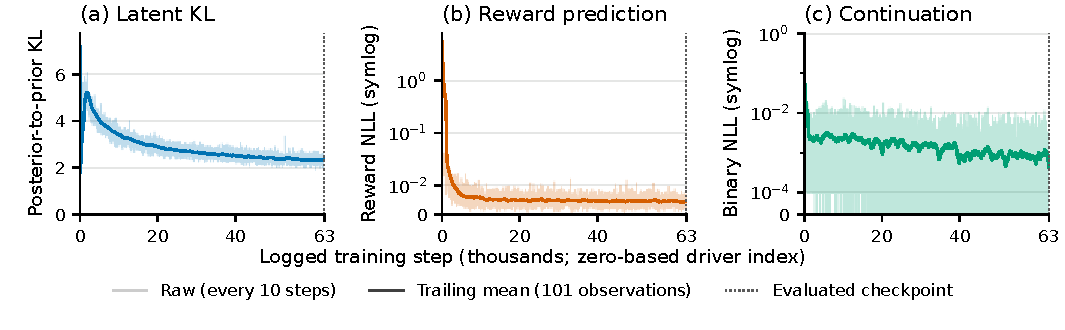
\includegraphics[width=\textwidth]{figures/dreamer_training_curves.pdf}
\caption{Training diagnostics for the evaluated \dreamer{} checkpoint,
recovered from the archived training log.  These are training-batch
quantities, not held-out losses and not match performance.  The axis is the
logged driver index, which is neither environment frames nor an exact count
of optimizer updates.  No comparable figure is shown for \lewm{} or \pets{}
because no usable scalar trace was archived for either: the 266 TensorBoard
event files found in the run directory contained only headers.  This is a
reproducibility gap in our setup, not a property of those methods.}
\label{fig:dreamer-curves}
\end{figure*}

\paragraph{Schedule.}
We report 45 completed rounds per matchup, for 135 rounds in total,
using the first three completed 15-round matches for each pair in scheduled
order.  Interrupted matches are excluded.  This rule also discards one
surplus match: the \dreamer{}--\pets{} pair completed a fourth match, which
\dreamer{} also won 15--0.  Counting it would make that pair 60--0 over
60 rounds and would not change any ordering; we drop it so that every pair
contributes the same number of rounds.  A fifth \dreamer{}--\pets{} match was
interrupted and is excluded under the same rule.
\lewm{} was always player 1 because its visual pipeline was validated only
from that perspective.  \dreamer{} and \pets{} played both sides against
each other, but not equally often in the selected matches.

\section{Results}
\label{sec:results}

Table~\ref{tab:results} summarizes the completed rounds.  \dreamer{} had the
best outcomes, but was not undefeated: \lewm{} won 13 rounds against it.
\lewm{} also won more rounds than \pets{}.  The 45--0
\dreamer{}--\pets{} result covers both player assignments.  No draws occurred.

\begin{table}[ht]
\centering
\caption{Completed outcomes from the first controller's perspective.
Each match is 15 rounds; matches are listed in scheduled order.}
\label{tab:results}
\small
\setlength{\tabcolsep}{4pt}
\begin{tabular}{lrrrrr}
\toprule
Matchup & M1 & M2 & M3 & Total & Win rate \\
\midrule
\dreamer{} vs.\ \lewm{} & 11--4 & 14--1 & 7--8 & 32--13 & 71.1\% \\
\lewm{} vs.\ \pets{} & 9--6 & 8--7 & 11--4 & 28--17 & 62.2\% \\
\dreamer{} vs.\ \pets{} & 15--0 & 15--0 & 15--0 & 45--0 & 100.0\% \\
\bottomrule
\end{tabular}
\end{table}

The per-match columns matter more than the totals.  The \dreamer{}--\lewm{}
pair is not a stable 71\% result: its three matches were 11--4, 14--1 and
7--8, so the third match was close to even while the second was nearly a
shutout.  Pooling them into 32--13 hides that spread.  The two other pairs
are internally consistent by comparison (\lewm{}--\pets{} at 9--6, 8--7,
11--4; \dreamer{}--\pets{} identical across all three).  The weights are the
same throughout; matches differ in random seed and, for \dreamer{}--\pets{},
in player assignment.  Seeding covers Python, NumPy and Torch only, so JVM
timing and concurrent scheduling remain uncontrolled and two matches at the
same seed need not agree.  With three matches per pair we cannot tell whether
the \dreamer{}--\lewm{} spread reflects seed sensitivity, within-match
drift, or JVM scheduling noise, and we do not fit a confidence interval to
three correlated observations.

Mean decision latency measured by the Python bridge was 9.3\,ms for
\dreamer{}, 70.3\,ms for \lewm{}, and 126.9\,ms for \pets{}; these are
per-decision means over the nine reported matches, weighted by each match's
decision count.  Only \dreamer{} usually met the nominal 60\,Hz budget of
16.67\,ms, exceeding it on 0.7\% of its 191,737 decisions.  \lewm{} and
\pets{} exceeded it on every one of theirs.
These timings do not establish real-time win rates, because the engine
waited for every decision.

\section{Limitations and Takeaway}

This is a small, descriptive experiment.  Pixel and state-vector inputs
provide different information; training data and compute budgets differ;
and \lewm{} is not side-balanced.  Exact synchronization of spectator
images with state callbacks was not verified.  All matches reuse the
same trained weights, and rounds within a game are correlated.  We therefore
do not treat the rounds as independent training runs or claim statistical
superiority, consistent with cautions about small-sample RL evaluation
\cite{agarwal2021precipice}.

For these checkpoints and this protocol, \dreamer{} achieved the strongest
combination of wins and decision speed, followed by \lewm{} in round
outcomes.  This does not isolate world-model quality.  A useful follow-up
would compare image-based \dreamer{} and \lewm{} on shared data, balance
player sides, and evaluate independently trained models under both lockstep
and real-time execution.  It should also anchor all three against the
platform's search-based sample agent \cite{yoshida2016mctsai}, which would
say whether any of these controllers is strong in absolute terms rather
than only relative to the other two, and run enough matches per pair to
characterize the seed-to-seed spread visible in Table~\ref{tab:results}.

\paragraph{Source code.}
\url{https://github.com/ThanhChinhBK/leworldgaming}.

{\footnotesize
\bibliographystyle{unsrtnat}
\bibliography{references}
}

\end{document}
